% !TeX root = Stageportfolio.tex



\begin{landscape}
	\subsubsection{Les 15}
	\begin{tabularx}{1.56\textwidth}{|p{0.35\textwidth}|X|}\hline
		\textbf{Administratieve gegevens}\newline\newline
		Kevin Truyaert\newline\newline
		technisch secundair onderwijs\newline
		3e graad, 1ste jaar, Techniek-Wetenschappen\newline
		VVKSO: \href{http://ond.vvkso-ict.com/leerplannen/doc/Toegepaste\%20fysica-2014-041.pdf}{http://ond.vvkso-ict.com/leerplannen /doc/Toegepaste\%20fysica-2014-041.pdf} \newline
		\underline{Lesonderwerp}:\newline Afwerken `Labo M4: De stroombalans' & \textbf{Doelstellingen}
		\begin{itemize}[itemsep=0.08\baselineskip]
			\item B24: De richting, de zin en de grootte van de Lorentzkracht op een rechte stroomvoerende geleider aangeven en hiermee de magnetische veldsterkte omschrijven. 
			\item AD4 Reflecteren: Over een waarnemingsopdracht/experiment/onderzoek en het resultaat reflecteren.
			\item AD5 Rapporteren: Over een waarnemingsopdracht/experiment/onderzoek en het resultaat rapporteren.
			\item AD10 Meettoestellen en meetnauwkeurigheid: De gepaste toestellen kiezen voor het meten van de behandelde grootheden en de meetresultaten correct aflezen en noteren.
			\item AD12 Grafieken: Meetresultaten grafisch voorstellen in een diagram en deze interpreteren.
		\end{itemize}
		\underline{Lesdoelen}\newline
		\vspace{-0.75cm}
		\begin{enumerate}[itemsep=0.08\baselineskip]
			\item De leerlingen kunnen de Lorentzkracht toepassen op de specifieke situatie van de stroombalans.
			\item De leerlingen reflecteren over de resultaten.
			\item De leerlingen rapporteren over hun resultaten.
			\item De leerlingen werken samen bij het opbouwen van hun verslag.
			\item De leerlingen houden bij hun berekeningen rekening met de nauwkeurigheid.
			\item De leerlingen stellen de meetresultaten grafisch voor.
			\item De leerlingen berekenen de magnetische veldsterkte van de magneet.
			\item De leerlingen begrijpen conceptueel wat de magnetische flux is.
			\item De leerlingen kunnen de drie factoren die de magnetische flux bepalen.
		\end{enumerate} \\\hline
	\end{tabularx}


	\begin{tabularx}{1.56\textwidth}{|p{0.55\textwidth}|X|}
		\hline
		\multirow{2}{0.55\textwidth}{\textbf{Beginsituatie}\newline  
		Er zijn acht leerlingen binnen 5TW. Er heerst een algemene klassfeer. De leerlingen hebben al theorie gekregen  rond en oefeningen gemaakt op de magnetische krachtwerking. \newline\newline De leerlingen hebben de week voor de krokusvakantie aan dit labo mogen beginnen en hebben toen de metingen uitgevoerd. Ze zijn ook al begonnen met de verwerking van hun data. \newline\newline Hannah was vorige les afwezig. Ik zal zorgen dat ze de opstelling nog even ziet voor ze de data van haar groepje verwerkt.   \newline\newline Mijn vorige lessen (11-12) zijn algemeen gezien goed verlopen. Dit labo mag drie lessen in beslag nemen en dit zal zeker lukken. Het begin van volgende laboles zal ik echter wel wat anders aanpakken. Ook in het algemeen zal ik mij wat meer op de zwakkere leerlingen in de groep moeten richten en de sterkere vooral zelfstandig laten bezig zijn, in plaats van extra verdiepende vragen aan die laatste groep te stellen.} & \textbf{Acties}\newline\newline  
		- \YellowHighlight{Ik herhaal de inhoud van het labo nog eens kort: waarover deden jullie onderzoek}{15cm}  \YellowHighlight{en wat waren de onderzoeksvragen?}{7cm} Door deze herhaling zorg ik ervoor dat de beginsituatie voor iedereen terug gelijk is en hoop ik dat de leerlingen terug kunnen inpikken na de krokusvakantie. \newline\newline
		- \GreenHighlight{Bij een labo is het de bedoeling om in groep een resultaat op de gestelde onderzoeks-}{15cm} \GreenHighlight{vragen te bekomen.}{3.6cm} Hier worden de leerlingen in drie groepen onder verdeeld. Hierdoor zal er een goede wisselwerking kunnen zijn tussen de leerlingen onderling en zijn er voldoende kritische blikken per groep om de vragen op te lossen. Tegelijkertijd kan ik als leerkracht vlot tussen de groepjes laveren wanneer ik zowel goede als minder goede zaken observeer.
		\newline\newline\newline\newline\newline
		
		\\ \cline{2-2}
		  & \textbf{Bronnen}\begin{itemize}
		  	\item Schramme, S. (2018) De stroombalans, labo magnetisme 4
		  	\item Frederiksen (2014), Current Balance 4565.00
		  \end{itemize}\\ \hline
	\end{tabularx}


\newpage
	
	\begin{tabularx}{1.56\textwidth}{|p{1.5cm}|p{9cm}|X|p{4cm}|}
		\hline
		\textbf{Nr. lesdoel } & \textbf{Inhoud (timing)}  & \textbf{Organisatie } & \textbf{Media } \\ \hline
		&\underline{Herhaling onderzoeksvragen} \underline{labo (10 minuten)}\newline De leerlingen nemen plaats aan hun computer en krijgen hun bundel terug. Daarna overloop ik via vraagstelling aan de leerlingen nog eens de onderzoeksvragen van het labo.
		&  \underline{Onderwijsleergesprek}\newline 
			De leerlingen krijgen hun bundel terug van mij en we overlopen de onderzoeksvragen van het labo nog even gezamenlijk. We gaan nog even dieper in op de effecten van de Lorentzkracht op de draad en de reactiekracht op de magneet. \newline\newline Ik overloop samen met Hannah de labobundel en overloop nog even kort met haar de theorie via onderwijsleergesprek (Hoe loopt de stroom, magnetisch veld, hoe is de Lorentzkracht gericht \ldots ) en bouw de opstelling. Samen testen we één configuratie en vraag ik wat er zou gebeuren wanneer de magneet omgekeerd zou staan.  De anderen werken ondertussen verder aan hun werkbundel.
		&  Labobundel
		\\ \hline
	\end{tabularx}\vspace{5mm}

\begin{tabularx}{1.56\textwidth}{|p{1.5cm}|p{9cm}|X|p{4cm}|}
	\hline
	\textbf{Nr. lesdoel } & \textbf{Inhoud (timing)}  & \textbf{Organisatie } & \textbf{Media } \\ \hline
	1\newline\newline 2\newline\newline 3\newline\newline 4\newline\newline 5\newline\newline 6\newline\newline 7&\underline{Afwerken laboverslag magnetisme 4:} \underline{de stroombalans (40 minuten)}\newline
	De leerlingen werken per groep verder aan hun individueel verslag. Ze  dienen individueel een verslag in, maar ze mogen nog met hun groepsleden samenwerken.
	&  \underline{Onderzoekspracticum}\newline De leerlingen zullen deze tijd nodig hebben om hun laboverslag af te werken. Ze zijn bezig met het afronden van onderdeel 6. Hierna bouwen ze een algemene conclusie op rond de Lorentzkracht, de stroomsterkte en de lengte van de geleider. Vanuit dit besluit, berekenen ze dan de veldsterkte van de magneet. Vijf van de acht leerlingen hebben op dit moment de fout gemaakt om niet met SI-eenheden te werken. Ik heb hier bewust nog niets over gezegd, zodat ze dit in hun besluit zullen ondervinden en bij zichzelf de vraag zullen moeten stellen wat er nu precies fout gelopen is.\newline\newline Hannah begint aan de dataverwerking met de data van het groepje waarbij ze ingedeeld zat. Ik probeer om extra bij haar langs te gaan.\newline\newline Iedereen dient hun verslag in de bundel in en zorgt ervoor dat hun dataverwerking in excel geüpload en geprint wordt. Indien er leerlingen vroeger klaar zijn, dan heb ik een bundel met extra oefeningen over de Lorentzkracht waar ze in groep kunnen aan werken. \newline\newline Op het eind van de les zeg ik hen nog eens dat ze morgen zeker hoofdstuk 5 moeten mee hebben.
	&  Computers (computerlokaal)\newline\newline Labobundel
	\\ \hline
\end{tabularx}


	
\end{landscape}


%\subsection*{Bijlage 5.1: slides introductie}

%
%\subsection*{Bijlage 1.2: bordschema theorie}
%\begin{center}
%	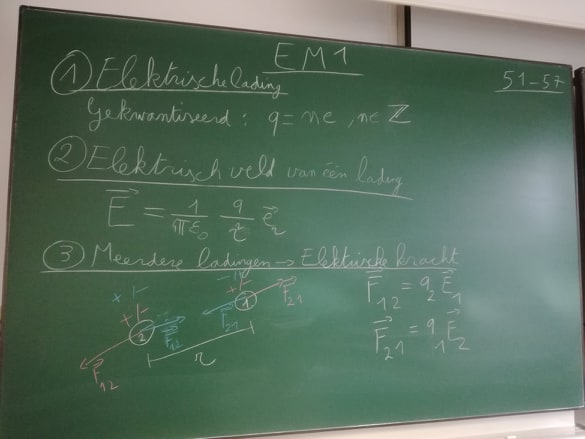
\includegraphics[width=0.9\textwidth]{Bord1a}
%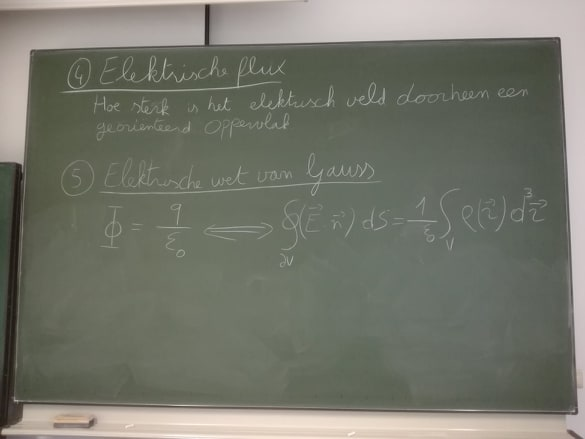
\includegraphics[width=0.9\textwidth]{Bord1b}
%\end{center}
%\newpage
%
%
%\includepdf[scale = 0.8,pages = 17,pagecommand=\subsection*{Bijlage 1.3: opgeloste oefeningen}]{Observaties_OpgelosteOef}
%\includepdf[scale = 0.8,pages =18-20,pagecommand=]{Observaties_OpgelosteOef}
%
%
%
%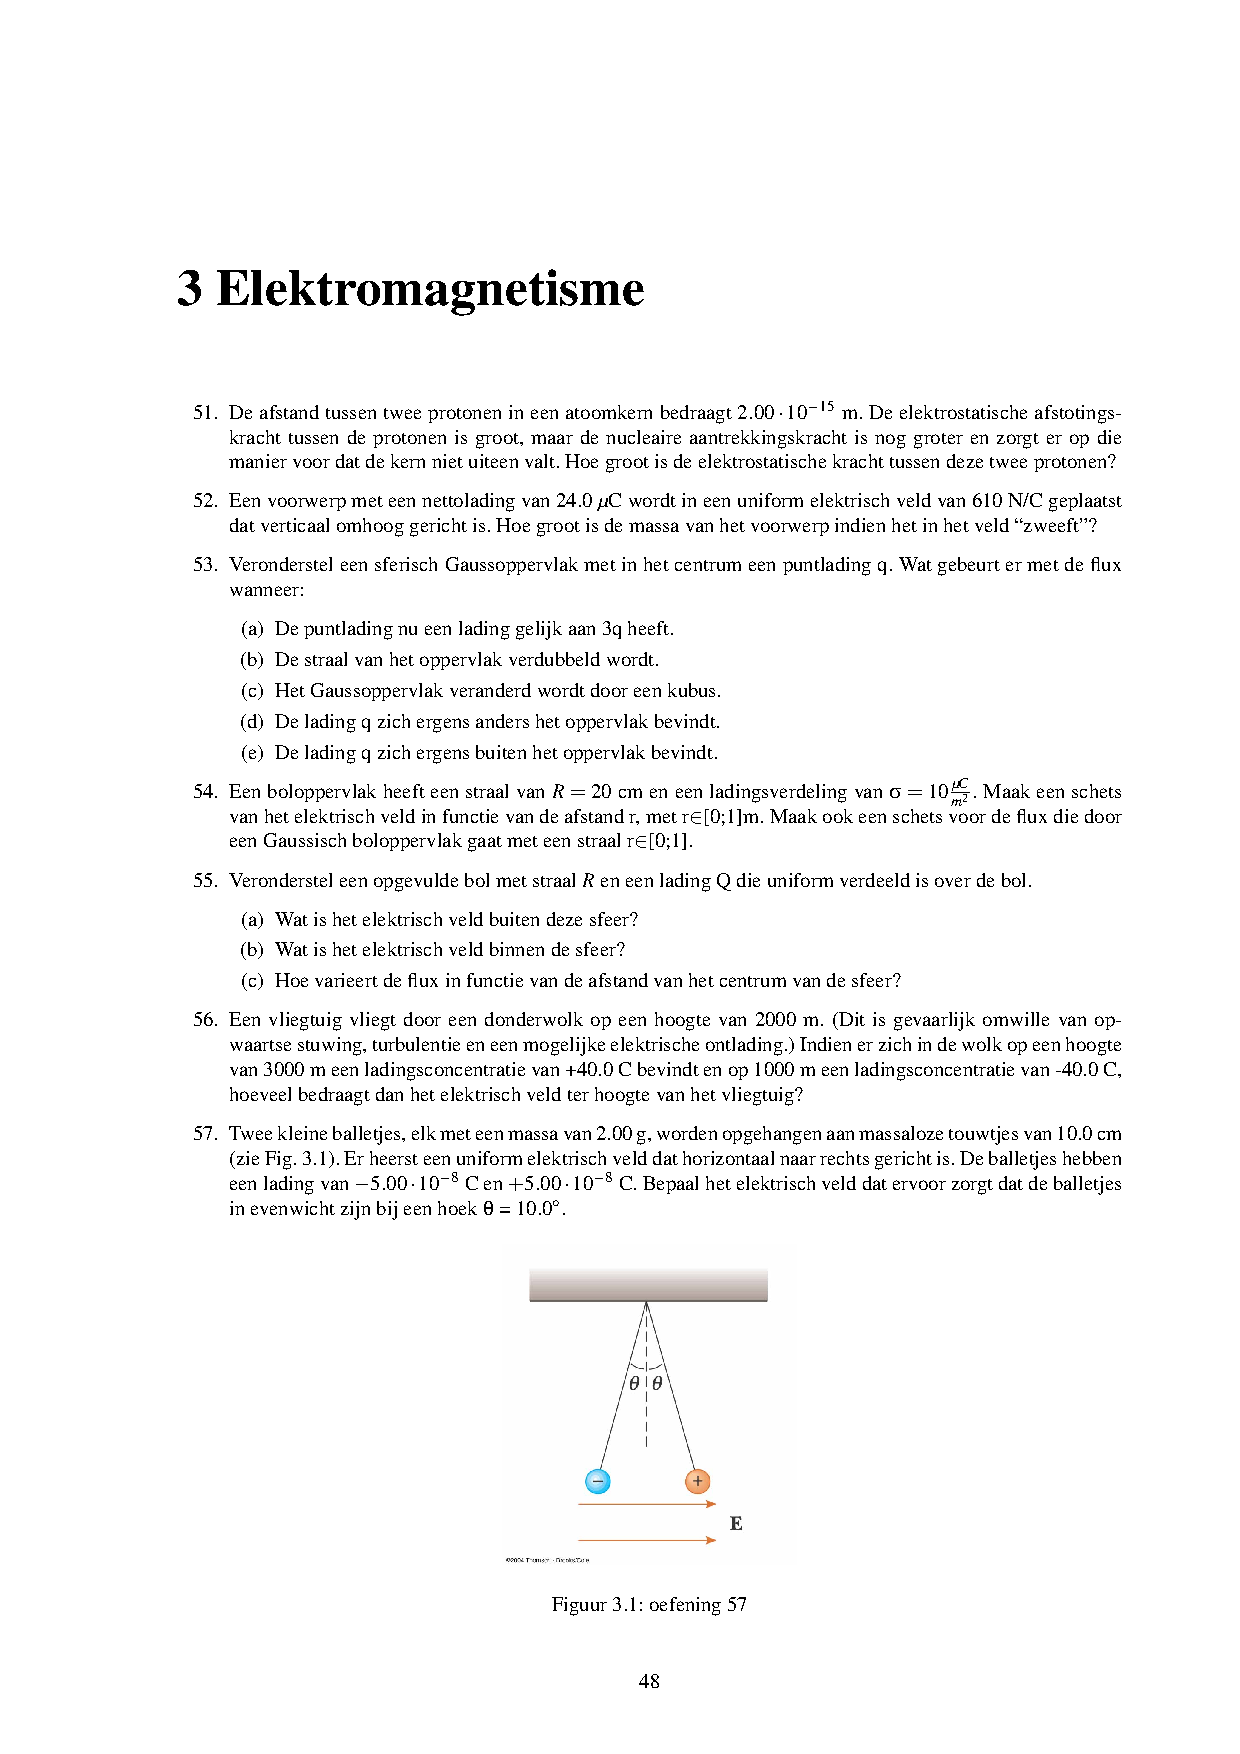
\includepdf[scale = 0.95,pages = 1,pagecommand=\subsection*{Bijlage 1.4: oefeningenbundel elektromagnetisme}]{OefeningenBundel}
%\includepdf[scale = 0.95,pages =2-,pagecommand=]{OefeningenBundel}